\documentclass[10pt]{article}

\usepackage[margin=1.15in]{geometry}
\usepackage[T1]{fontenc}
\usepackage[utf8]{inputenc}
\usepackage{microtype}
% amsmath/amssymb/amsthm must load before newtxmath, otherwise both try to
% define \Bbbk and \openbox and the build errors out.
\usepackage{amsmath, amssymb, amsthm}
\usepackage{newtxtext}
\usepackage{newtxmath}
\usepackage{booktabs}
\usepackage{graphicx}
\graphicspath{{../assets/figures/}}
\usepackage{subcaption}
\usepackage{caption}
\usepackage{enumitem}
\usepackage{xcolor}
\usepackage{hyperref}

\hypersetup{
  colorlinks=true,
  linkcolor=blue!45!black,
  citecolor=blue!45!black,
  urlcolor=blue!45!black
}

\setlength{\parindent}{1.2em}
\setlength{\parskip}{0.25em}
\setlist[itemize]{leftmargin=1.2em, itemsep=0.15em, topsep=0.15em}
\setlist[enumerate]{leftmargin=1.4em, itemsep=0.15em, topsep=0.15em}
\renewcommand{\arraystretch}{1.1}

% --- Convenience macros ---
\newcommand{\appref}[1]{(Appendix~#1)}
\newcommand{\figref}[1]{Fig.~#1}

\title{\vspace{-1.2em}
Algorithm or Skill?\\
\large A Monte Carlo Simulation of Creator Strategy and Emergent Inequality on TikTok}
\author{Rayyan Maan}
\date{April 2026}

\begin{document}
\maketitle
\thispagestyle{plain}

\noindent\textbf{Code and reproducibility.}
All simulation code, calibration steps, and figure-generation scripts live in the companion
notebook \texttt{notebooks/creator\_strategy\_simulation.ipynb}, alongside an installable package
(\texttt{src/creator\_strategy\_sim/}) and a test suite that reproduces every calibration constant
quoted below. Repository: \href{https://github.com/rayyanmaan/tiktok-creator-strategy-simulation}{\texttt{github.com/rayyanmaan/tiktok-creator-strategy-simulation}}.

\tableofcontents
\vspace{0.5em}

\section{Scenario description}
\subsection{Motivation and research question}
TikTok is unusual among major platforms because early distribution does not require an existing follower base. A new video is typically routed to an initial cohort of users before any explicit social-graph signal can matter. In that setting, it is not obvious whether ``content strategy'' is actually decisive, or whether early exposure randomness dominates outcomes.

This project asks a narrow counterfactual question: across a distribution of simulated platform environments, does a creator's strategy---niche consistency, trend chasing, quality investment, or random posting---produce meaningfully different follower outcomes and virality outcomes? If mean growth is similar across strategies, does strategy still determine the \emph{mechanism} of growth?

Simulation is the right tool for two reasons. First, strategies cannot be randomly assigned to real creators in a controlled trial. Second, TikTok's recommendation system is not publicly specified at the implementation level, so any empirical-only approach is forced to treat the platform as a black box. A calibrated simulation allows holding all non-strategy choices fixed and varying only strategy, which is the comparison the report is built around \appref{A2}.

From a talent-management perspective, the question becomes operational: should an agency advise clients to post consistently in a niche, chase trends aggressively, invest in production quality, or simply post without a coherent plan? The goal here is not to claim a universal rule for all creators, but to make the model's implied trade-offs explicit and check whether they are statistically stable under Monte Carlo uncertainty.

\subsection{Data sources and what each one contributes}
This model is calibrated from four sources \appref{A1}:

\paragraph{BrightData TikTok user profiles (CSV; 1{,}000 creators).}
After cleaning, all 1{,}000 rows are retained \appref{A1a}. The follower distribution is extremely heavy-tailed (range 1 to 14{,}500{,}000), and the implied inequality is high: the Gini coefficient is \(G_{\text{real}} = 0.9086\) \appref{A1a}. That value becomes an external calibration target for inequality; the simulation should reproduce heavy tails and a strongly concave Lorenz curve, even if it cannot match the extreme tail perfectly at small simulated population sizes.

\paragraph{TikTok popular hashtag dataset (XLSX; 1{,}200 videos).}
This dataset provides play counts, likes, and shares per video keyed by hashtag topic \appref{A1b}. After filtering for minimum topic support, 12 topics remain (humor-adjacent categories dominate). I compute topic-specific like-rate and share-rate multipliers and use them as content-topic engagement multipliers in the recommendation funnel. The cross-topic baseline like-rate is 0.1478 and the baseline share-rate is 0.0041 \appref{A1b}. These rates are scaled (LIKE\_SCALE \(=35.0\), SHARE\_SCALE \(=21.0\)) so that an average-quality video (\(q=0.5\)) has mean engagement score \(E \approx 0.32\), slightly below the amplification threshold \(0.35\); that choice makes virality feasible but not guaranteed, which is necessary for strategy trade-offs to exist \appref{A1b}.

\paragraph{Google Trends fits for four TikTok-native trends.}
Four trends (Sea Shanty, Corn Kid, Brat Summer, Demure) are used to fit log-normal lifecycle curves, producing four \((\mu,\sigma)\) pairs \appref{A1c}. The trend engine samples one pair uniformly at random when a new trend spawns, replacing an arbitrary decay schedule with a data-grounded family of lifecycle shapes.

\paragraph{HypeAuditor 2026 benchmarks.}
HypeAuditor provides a realistic tier distribution (nano/micro/mid/macro/mega) and engagement benchmarks by tier \appref{A1d}. This is used to initialize creator follower counts in a way that reflects the actual creator population composition, rather than starting everyone at zero.

\subsection{What the simulation measures}
Each Monte Carlo run simulates \(N_{\text{creators}} = 30\) creators for \(T = 60\) weekly time steps \appref{A0}. Each strategy is evaluated over \(N_{\text{MC}}=1{,}000\) independent runs \appref{A6--A11}.

Outputs (with units and definitions):
\begin{itemize}
  \item \textbf{Final followers} \(F_i(T)\) per creator; the report often uses the \emph{run-level mean} \(\bar{F}(T)\) across 30 creators \appref{A6}.
  \item \textbf{Survival rate}: fraction of runs where \(\bar{F}(T) > \bar{F}(0)\) \appref{A7}.
  \item \textbf{Viral rate}: fraction of videos with engagement score \(E > \theta\), averaged within-run then across runs \appref{A8}.
  \item \textbf{Gini coefficient} of the within-run follower distribution across 30 creators, averaged across runs \appref{A9}.
  \item \textbf{Q4/Q1 viral-rate ratio}: within each strategy, runs are binned into quartiles by final followers; the ratio compares mean viral rates in top vs.\ bottom quartiles \appref{A8b}.
  \item \textbf{Engagement score} \(E\): a weighted sum of completion, shares, likes, and skips (defined below) \appref{A2b}.
\end{itemize}

\subsection{Model structure and rules}
The model has three interacting components \appref{A2}: creator agents, a recommendation funnel, and a trend engine. The intent is not to reproduce TikTok's full ranking stack, but to implement a minimal feedback loop that (i) provides baseline exposure to all creators, (ii) amplifies content that clears an engagement threshold, and (iii) allows strategies to change how often a creator aligns with trends and how much they trade quality for speed.

\subsubsection{Creator agents}
Each creator \(i\) is assigned a fixed strategy that sets a quality distribution and behavior parameters at initialization \appref{A2a}. Quality \(q_i\) is drawn once from a Normal distribution and clipped to \([0.05,1.0]\). This is a deliberate choice: by keeping quality fixed within-run, the experiments isolate strategy differences from learning effects.

Each creator also has a content-topic distribution \(C_i(t)\) over \(K=12\) topics (from the hashtag dataset). Trend-adapting strategies update their content vector toward the active trend topic:
\[
C_i(t+1) = \bigl(1-\eta\,I(t)\bigr)\,C_i(t) + \eta\,I(t)\,e_{\text{trend}},
\]
where \(I(t)\in[0,1]\) is trend intensity and \(e_{\text{trend}}\) is the one-hot trending topic \appref{A2a}. Niche specialists have \(\eta=0\), so \(C_i\) is stable by construction; this is verified by a unit test \appref{A3}.

\paragraph{Strategy parameterization.}
The four strategies are parameterized as follows \appref{A2a}:
\begin{center}
\small
\begin{tabular}{lcccccc}
\toprule
Strategy & \(\mu_q\) & \(\sigma_q\) & \(\eta\) & \(\tau\) & posting rate \\
\midrule
Niche Specialist & 0.58 & 0.07 & 0.00 & 0.00 & 2 \\
Trend Chaser & 0.30 & 0.18 & 0.55 & 0.90 & 3 \\
Quality-Focused & 0.88 & 0.03 & 0.08 & 0.08 & 1 \\
Random Baseline & 0.45 & 0.22 & 0.28 & 0.38 & 2 \\
\bottomrule
\end{tabular}
\end{center}
Quality-focused creators have high mean quality and low variance (consistency). Trend chasers have low mean quality and high variance (speed-driven volatility) but high trend sensitivity and high posting volume. Niche specialists do not pivot by definition. The random baseline is a null strategy intended to sit between structured approaches.

\subsubsection{Recommendation algorithm: a two-stage funnel}
Each video is shown to an initial cohort of users before any amplification decision \appref{A2b}. The initial cohort size is a Poisson draw with mean \(N_{\text{test}}=100\), which represents irreducible exposure luck.

For each user-view, four engagement events are sampled stochastically with probabilities driven by creator quality and topic multipliers \appref{A2b}. The engagement score is then computed as
\[
E \;=\; 0.40\,\widehat{p}_{\text{complete}} \;+\; 0.25\,\widehat{p}_{\text{share}} \;+\; 0.20\,\widehat{p}_{\text{like}} \;-\; 0.15\,\widehat{p}_{\text{skip}},
\]
where hats denote empirical rates in the initial cohort. Completion is weighted most heavily, shares next, then likes, with skips penalizing the score. These weights are architectural choices motivated by watch-time priority; they are not estimated from data, and I treat them as part of the model definition rather than a tuned parameter.

Amplification is threshold-based: if \(E>\theta\) with \(\theta=0.35\), impressions expand:
\[
\text{impressions} \;=\; \text{initial} \cdot \bigl(1+\alpha(E-\theta)\bigr),\quad \alpha=8.0,
\]
otherwise the video receives no additional distribution \appref{A2b}. New followers are a fixed fraction of impressions (conversion rate \(=0.02\)). A weekly churn term removes \(0.3\%\) of current followers, preventing unlimited growth and representing baseline audience decay \appref{A2b}.

\subsubsection{Trend engine}
At each step, a new trend spawns with probability \(p_{\text{trend}}=0.12\) in the main experiments \appref{A6}. When a trend spawns, its lifecycle intensity curve is sampled from the empirical \((\mu,\sigma)\) pairs fitted from Google Trends \appref{A1c}. For simplicity, trends do not overlap: at most one trend is active at a time.

\subsection{Key modeling assumptions}
The model is intentionally minimal, so assumptions matter. The most important are \appref{A1--A2}:
\begin{enumerate}
  \item \textbf{Quality is fixed within-run.} This isolates strategy effects but prevents learning or skill acquisition.
  \item \textbf{Users are not individual agents.} The model samples engagement from distributions instead of simulating social networks; it cannot represent community-driven cascades.
  \item \textbf{Single active trend.} This approximates a dominant trend regime but excludes overlapping cultural moments.
  \item \textbf{Threshold amplification.} This captures a feedback loop but is not meant as a literal description of TikTok's ranking system.
  \item \textbf{No creator-creator interactions.} There are no collaborations or cross-promotion dynamics; the model is closest to nano/micro creator settings.
\end{enumerate}

\section{Theoretical analysis}
The goal of this section is to treat the simulation as a stochastic process with analyzable components, then use theory as a benchmark for what the Monte Carlo runs should do.

\subsection{Virality probability: expectation, variance, and a normal approximation}
In the initial cohort, each engagement component is an empirical average of Bernoulli trials. For a component \(j\in\{\text{complete, share, like, skip}\}\) and \(n\) users,
\[
\widehat{p}_j \;=\; \frac{1}{n}\,\text{Binomial}(n,p_j),\qquad
\mathbb{E}[\widehat{p}_j]=p_j,\qquad
\mathrm{Var}(\widehat{p}_j)=\frac{p_j(1-p_j)}{n}.
\]
By linearity of expectation,
\[
\mathbb{E}[E] \;=\; 0.40\,p_{\text{complete}} + 0.25\,p_{\text{share}} + 0.20\,p_{\text{like}} - 0.15\,p_{\text{skip}}.
\]
If user responses are treated as independent within the initial cohort (the assumption used in Appendix A5), then
\[
\mathrm{Var}(E)\;=\;\sum_{j} w_j^2\,\mathrm{Var}(\widehat{p}_j),
\]
with weights \(w_j\in\{0.40,0.25,0.20,0.15\}\) (skip uses \(+0.15\) in variance because the sign disappears).

Because \(n=100\) and \(E\) is a weighted sum of scaled binomials, Appendix A5 uses a normal approximation for the viral probability:
\[
\mathbb{P}(\text{viral}) \;=\; \mathbb{P}(E>\theta) \;\approx\; 1-\Phi\!\left(\frac{\theta-\mathbb{E}[E]}{\sqrt{\mathrm{Var}(E)}}\right),
\]
where \(\Phi\) is the standard normal CDF \appref{A5}.

Evaluating at the strategy mean quality values yields the analytical predictions \appref{A5}:
\begin{center}
\small
\begin{tabular}{lcc}
\toprule
Strategy & \(q=\mu_q\) & Theory \(P(\text{viral})\) \\
\midrule
Niche Specialist & 0.58 & 0.0703 \\
Trend Chaser & 0.30 & \(\approx 0.0000\) \\
Quality-Focused & 0.88 & \(\approx 1.0000\) \\
Random Baseline & 0.45 & \(\approx 0.0000\) \\
\bottomrule
\end{tabular}
\end{center}

The point of this table is not that it matches perfectly (it does not), but that it provides a crisp baseline for interpreting the Monte Carlo results in \figref{8} \appref{A8}.

\subsection{Expected follower growth rate and why it under-predicts the simulation}
In a simplified zero-initial-followers world, the expected follower increment per step for creator \(i\) can be sketched as
\[
\mathbb{E}[\Delta F_i] \;\approx\; r_i \cdot \mathbb{P}(\text{viral}\mid q_i)\cdot \mathbb{E}[\text{impressions}\mid \text{viral}] \cdot \rho,
\]
where \(r_i\) is posting rate, \(\rho=0.02\) is conversion rate, and the impressions term comes from the amplification mapping \appref{A2b}. Appendix A5 computes strategy-level expected increments using approximations for \(\mathbb{E}[E\mid E>\theta]\) and finds very small totals over 60 steps (order \(10^1\) to \(10^2\) followers) \appref{A5}.

The Monte Carlo experiments report mean final follower counts around 13{,}280--13{,}350 for all strategies \appref{A6}. This is not a numerical glitch; it is a modeling consequence of initialization. The simulation does not start creators at zero. It draws initial followers from a realistic tier distribution (dominated by nano creators with nontrivial existing follower counts) \appref{A1d, A2d}. Once follower stock is large at \(t=0\), the model's churn and growth terms mainly govern deviations around that stock, and the run-level mean \(\bar{F}(T)\) becomes relatively insensitive to strategy choices that act through virality. In other words: the theoretical calculation describes incremental growth from a small baseline, but the simulation operates in a regime where baseline follower stock and churn balance dominate the final mean.

\subsection{Why follower distributions tend toward log-normality}
Follower growth in the simulation is effectively multiplicative: followers carry over from one step to the next with small random increments and decrements. A common argument is that if
\[
F(t+1) = F(t)\,(1+\delta_t),
\]
then
\[
\log F(T) = \log F(0) + \sum_{t=0}^{T-1} \log(1+\delta_t),
\]
and if the \(\log(1+\delta_t)\) terms have finite variance and weak dependence, the sum is approximately normal by a CLT heuristic, making \(F(T)\) approximately log-normal \appref{A5}. For a log-normal distribution with log-std \(\sigma_{\log F}\), the Gini coefficient has closed form:
\[
G \;=\; 2\Phi\!\left(\frac{\sigma_{\log F}}{\sqrt{2}}\right) - 1.
\]
Appendix A9 uses this as a theoretical comparator, then checks it against simulated and real inequality.

\subsection{Recovery time after a trend}
Trend adaptation can be summarized by a simple decay argument. If a trend chaser drifts toward a trend topic by an amount \(d_0\) and then the trend ends, the residual drift decays geometrically:
\[
d(k)=d_0\,(1-\eta)^k.
\]
Solving for the time to return below a tolerance \(\varepsilon\) gives
\[
k^\star = \frac{\log(\varepsilon/d_0)}{\log(1-\eta)}.
\]
With \(\eta=0.55\), \(d_0=0.8\), and \(\varepsilon=0.05\), this yields \(k^\star \approx 3.5\) weeks \appref{A5}. This calculation is not a separate experiment in the final notebook, but it is useful for interpreting why the trend chaser can be resilient even when its per-video quality is low: aggressive adaptation implies fast post-trend re-alignment.

\section{Implementation and correctness}
\subsection{Code architecture}
The notebook is organized so that each modeling component is implemented once and then re-used across experiments \appref{A2}. The code is structured around four classes:
\begin{itemize}
  \item \textbf{Creator} stores agent state (quality, content vector, posting policy) and produces videos \appref{A2a}.
  \item \textbf{Algorithm} implements the initial-cohort evaluation and threshold amplification \appref{A2b}.
  \item \textbf{TrendEngine} manages trend arrival and intensity through time \appref{A2c}.
  \item \textbf{Simulation} orchestrates the weekly loop and records outcomes \appref{A2d}.
\end{itemize}
Experiments call a single Monte Carlo runner, \texttt{run\_monte\_carlo()}, which standardizes seeds, run counts, and output storage \appref{A2e}. This matters for readability: strategy comparisons are implemented as a loop over strategy keys instead of separate scripts, which reduces the risk of silent divergence across experimental conditions.

\subsection{Correctness tests}
Appendix A3 implements five unit tests that check monotonicity, initialization, and strategy-specific invariants \appref{A3}. All five pass in the final notebook run.

The most informative test is the monotonicity check: engagement score \(E\) increases smoothly with quality, and the mean \(E\) crosses the amplification threshold near \(q\approx 0.55\) \appref{A3}. This anchors interpretation later: strategies with \(\mu_q\) below 0.55 should rarely go viral without a trend boost, while strategies above 0.55 should go viral regularly. The visualization from that test is included as \figref{4}.

\begin{figure}[t]
  \centering
  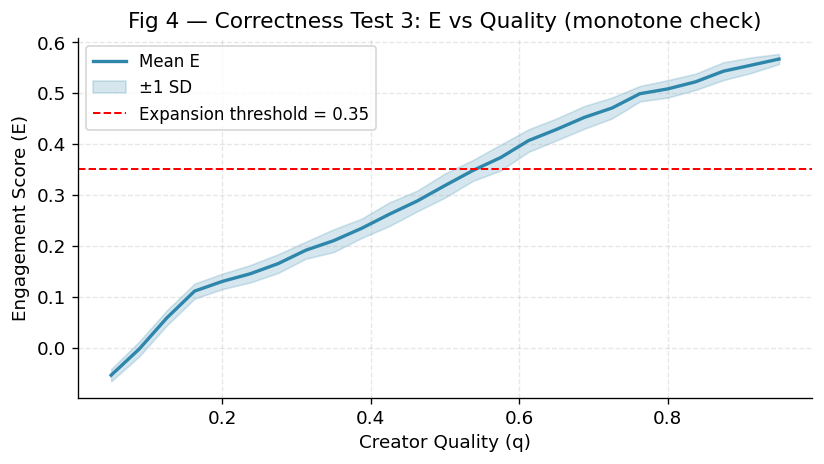
\includegraphics[width=0.72\linewidth]{fig4_correctness_quality.png}
  \caption{\textbf{Engagement score monotonicity check.} Mean engagement score increases with creator quality and crosses the amplification threshold around \(q\approx 0.55\). This validates that the funnel has a stable quality signal rather than noisy or inverted behavior \appref{A3}.}
  \label{fig:fig4}
\end{figure}

\section{Empirical analysis and results}
This section builds in a specific order: first, calibration results that ground the model; then a single-run visualization that provides qualitative intuition; then the Monte Carlo experiments that answer the research question.

\subsection{Calibration results}
\paragraph{Real follower inequality.}
From the BrightData creator sample, \(G_{\text{real}}=0.9086\) \appref{A1a}. The Lorenz curve is extremely concave: the cumulative share of followers remains near zero for most of the creator percentiles and rises sharply near the top tail. This is the inequality target against which the simulation is compared in Experiment 4.

\paragraph{Topic multipliers.}
The hashtag dataset produces topic multipliers for like rates and share rates \appref{A1b}. Like multipliers are ordered in the plot so that longer horizontal bars indicate higher multipliers; topics like \texttt{jokes} and \texttt{lmao} are among the largest (blue), while \texttt{fun} and \texttt{funny} are among the smallest (red). Share multipliers have a different ranking: \texttt{memes} is the largest (around 1.3), with \texttt{humor} and \texttt{lmao} around 1.2, while \texttt{fun} and \texttt{love} are the smallest \appref{A1b}. This mismatch is useful: it prevents the model from collapsing topic choice into a single scalar ``good topic'' dimension.

\paragraph{Trend lifecycle fits.}
The log-normal fits track the overall trend arcs reasonably well, including Demure's rapid rise and fall; for Sea Shanty, Corn Kid, and Brat Summer the fitted curves capture the broad pattern but miss sharp local peaks \appref{A1c}. In this model, that mismatch is acceptable because the trend engine uses the fitted curves as a family of plausible intensity schedules rather than requiring exact reconstruction of each trend.

\begin{figure}[t]
  \centering
  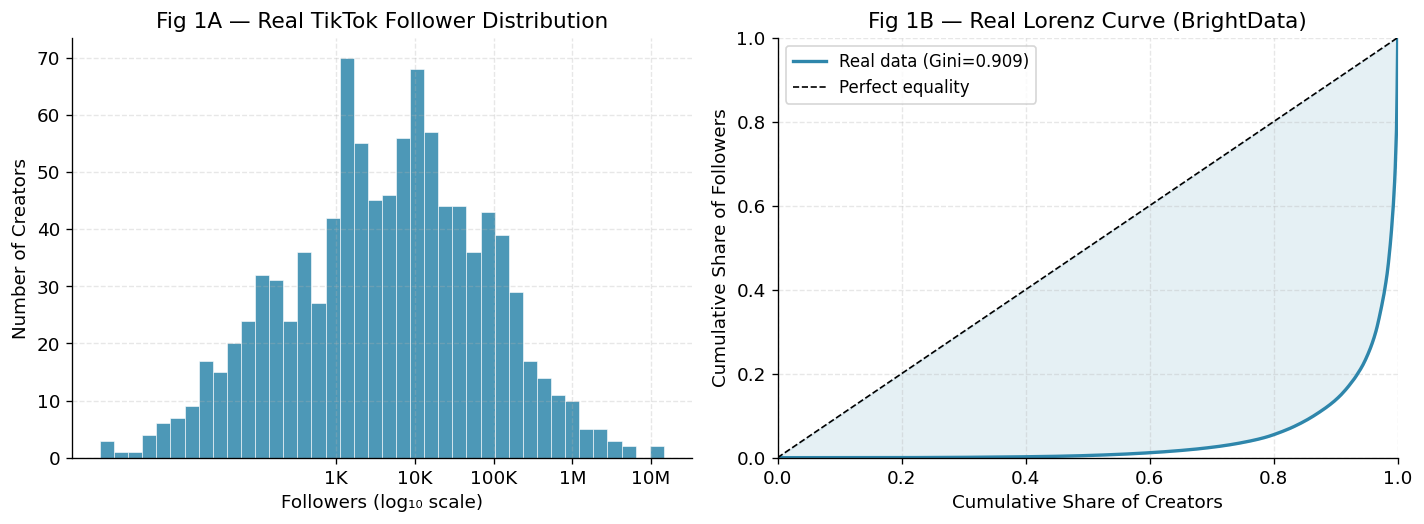
\includegraphics[width=0.98\linewidth]{fig1_follower_distribution.png}
  \caption{\textbf{Real-data calibration target.} The BrightData sample has extreme follower inequality, summarized by \(G_{\text{real}}=0.9086\). The Lorenz curve remains close to the x-axis for most percentiles, then rises sharply in the top tail \appref{A1a}.}
  \label{fig:fig1}
\end{figure}

\begin{figure}[t]
  \centering
  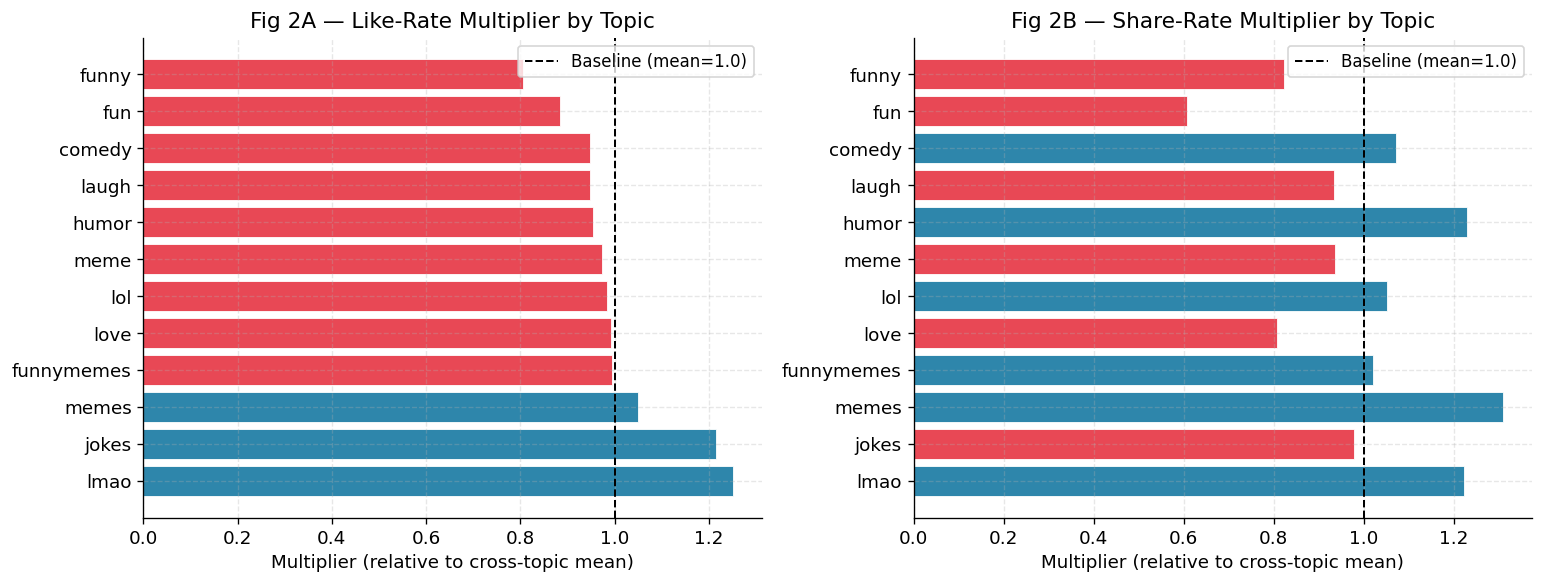
\includegraphics[width=0.98\linewidth]{fig2_topic_engagement.png}
  \caption{\textbf{Content-topic engagement multipliers.} Like-rate multipliers are visually ordered (longer bars indicate larger multipliers); share multipliers have a different topic ranking. These multipliers are used directly in the engagement probability functions \appref{A1b}.}
  \label{fig:fig2}
\end{figure}

\begin{figure}[t]
  \centering
  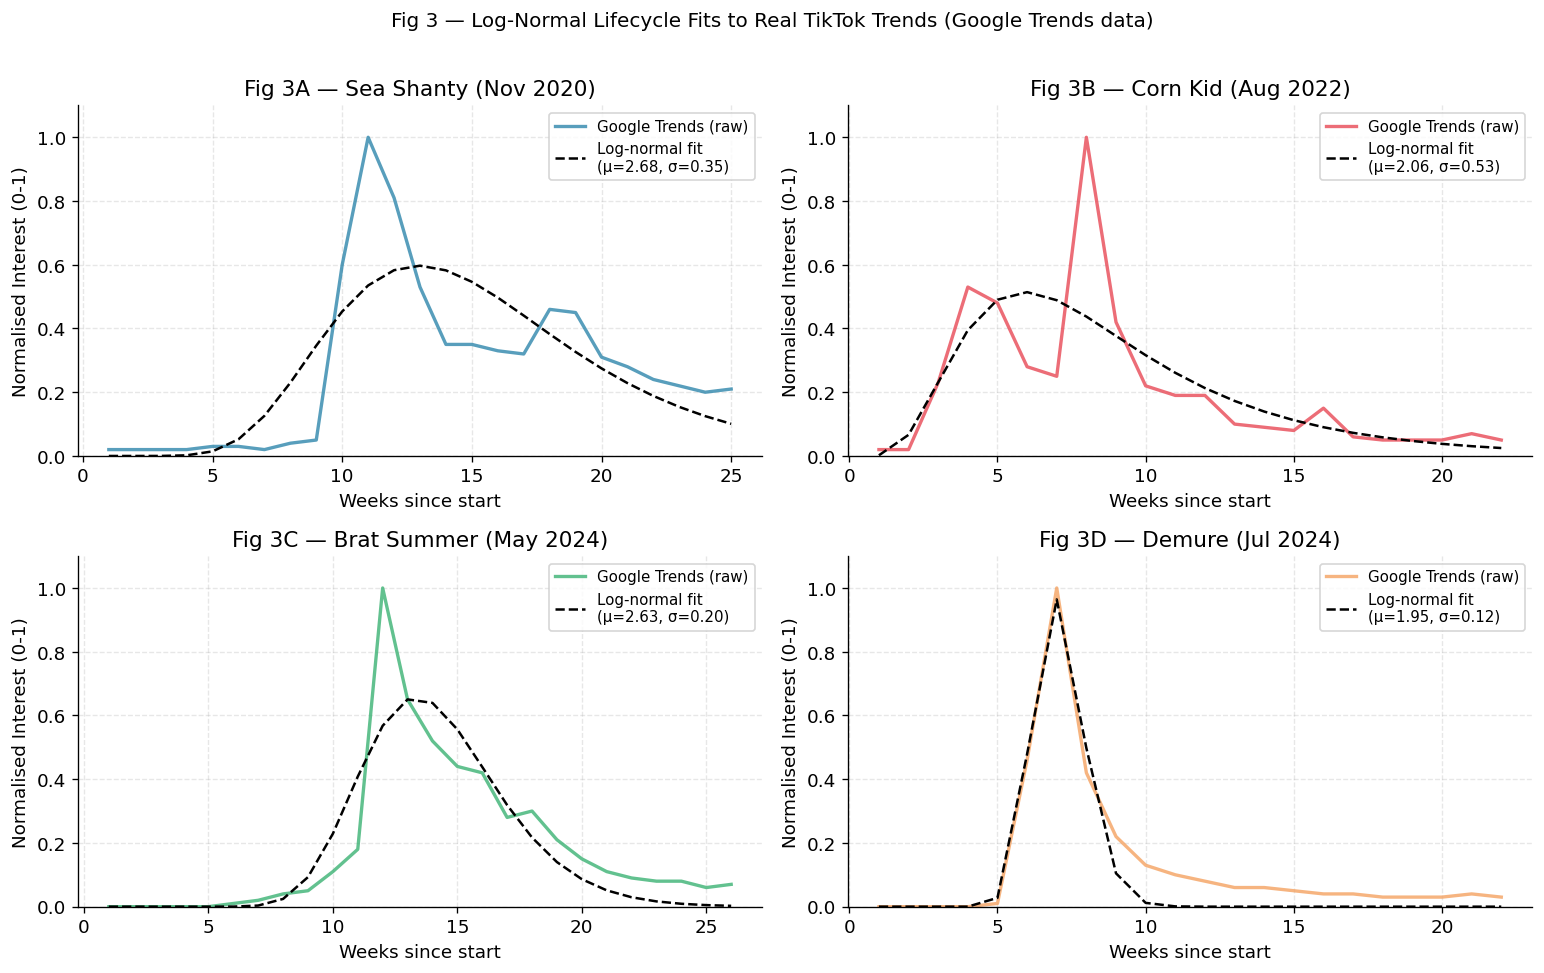
\includegraphics[width=0.92\linewidth]{fig3_trend_fits.png}
  \caption{\textbf{Empirical trend lifecycles.} Four fitted log-normal curves provide a distribution of plausible trend shapes (flash-viral to sustained). The trend engine samples from these fitted parameter pairs when spawning new trends \appref{A1c}.}
  \label{fig:fig3}
\end{figure}

\subsection{Single-run visualization}
The animation in Appendix A4 (saved as \texttt{fig5\_animation.gif}) provides a sanity check for the time dynamics \appref{A4}. In the final frame at \(T=60\), all strategies decline slowly from around 5{,}100 followers, with the trend chaser declining slowest and thus ending highest; quality-focused is next; niche and random are below and close together. This is consistent with a regime where weekly churn is strong relative to net gains from amplification, and where the trend chaser's higher posting volume provides more opportunities to offset churn.

\begin{figure}[t]
  \centering
  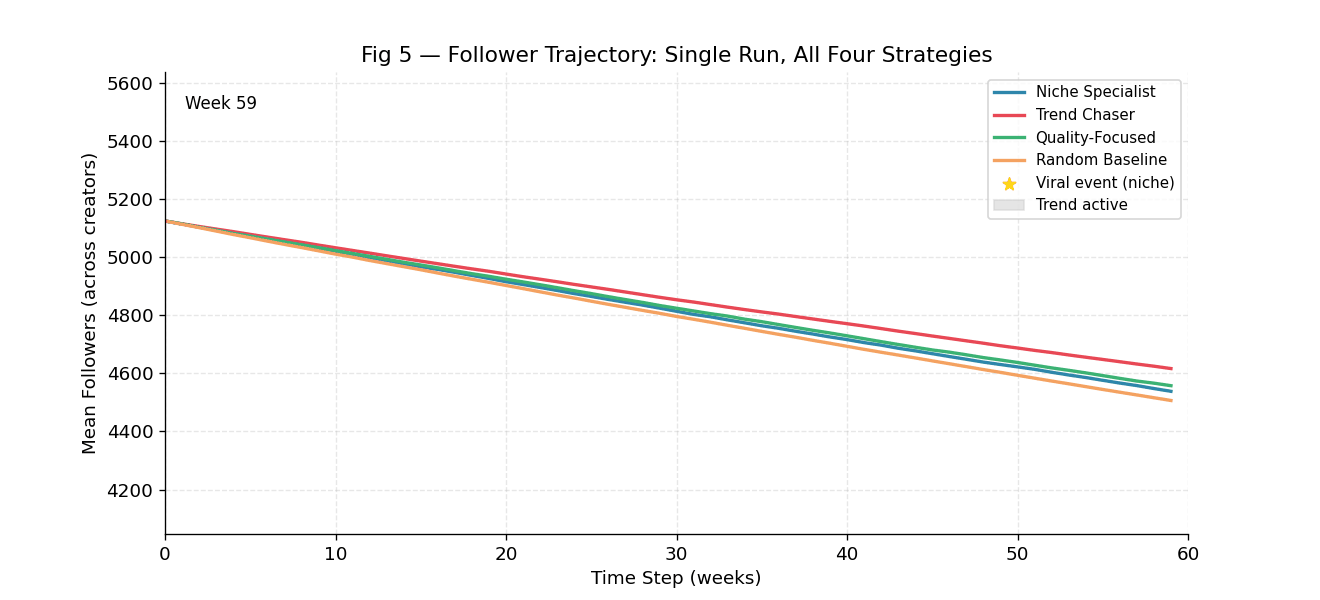
\includegraphics[width=0.95\linewidth]{fig5_animation_final_frame.png}
  \caption{\textbf{Qualitative trajectory check.} In a representative single run, all strategies drift downward over 60 weeks, with the trend chaser declining slowest and ending highest. Trend windows appear as background bands in the animation \appref{A4}.}
  \label{fig:fig5}
\end{figure}

\subsection{Experiment 1: follower growth distributions}
Experiment 1 runs 1{,}000 Monte Carlo trials per strategy and records the run-level mean final followers across 30 creators \appref{A6}. The resulting histograms are nearly indistinguishable across strategies: means fall in a narrow band (about 13{,}281--13{,}351), medians cluster around 9{,}559--9{,}625, and higher moments (standard deviation and skewness) are effectively identical across strategies \appref{A6}. The confidence intervals for the mean overlap heavily \appref{A11}. This is the central null result on magnitude: in this modeled regime, strategy does not move the average final-follower metric in a meaningful way.

\begin{figure}[t]
  \centering
  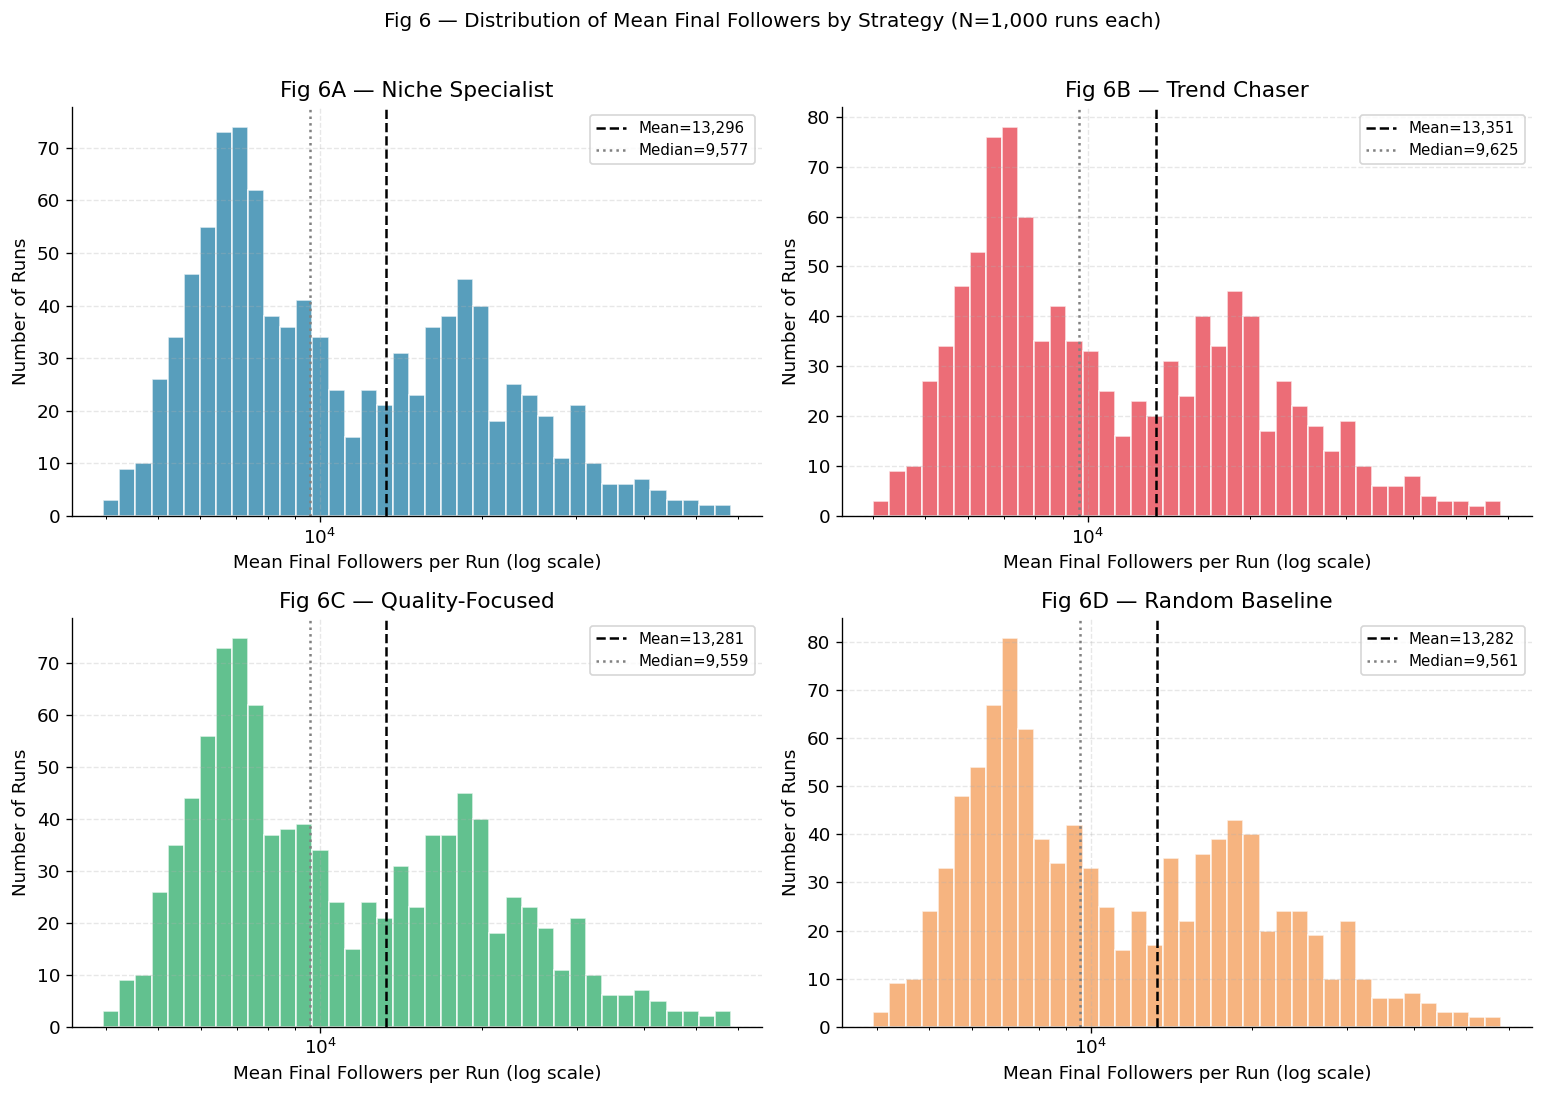
\includegraphics[width=0.92\linewidth]{fig6_follower_histograms.png}
  \caption{\textbf{Follower outcome distributions are nearly identical.} Across 1{,}000 runs per strategy, the four histograms align closely in center and spread. This supports the claim that in this model, mean follower magnitude is dominated by initialization and churn dynamics rather than strategy \appref{A6, A11}.}
  \label{fig:fig6}
\end{figure}

\subsection{Experiment 2: survival rate and downside risk}
To measure downside risk, I define \emph{survival} as a run where the creator population ends with higher mean followers than it started: \(\bar{F}(T)>\bar{F}(0)\) \appref{A7}. Survival rates are low for all strategies (6--11\%), implying that churn dominates in most simulated environments. The ranking is nonetheless clear:
\[
\text{Trend Chaser } 0.1056 \;>\; \text{Niche } 0.0735 \;>\; \text{Random } 0.0655 \;>\; \text{Quality-Focused } 0.0640,
\]
with non-overlapping confidence intervals for the top-vs-bottom comparison \appref{A7, A11}.

This ordering is counterintuitive if one thinks of quality as the only driver of growth. In the model, posting rate matters mechanically because each posted video draws a new initial cohort and has an independent chance to clear the amplification threshold. The trend chaser posts three times per step (vs.\ one for quality-focused) and has high trend sensitivity, so even a low per-video viral probability can accumulate enough amplified impressions over time to offset churn more reliably.

\begin{figure}[t]
  \centering
  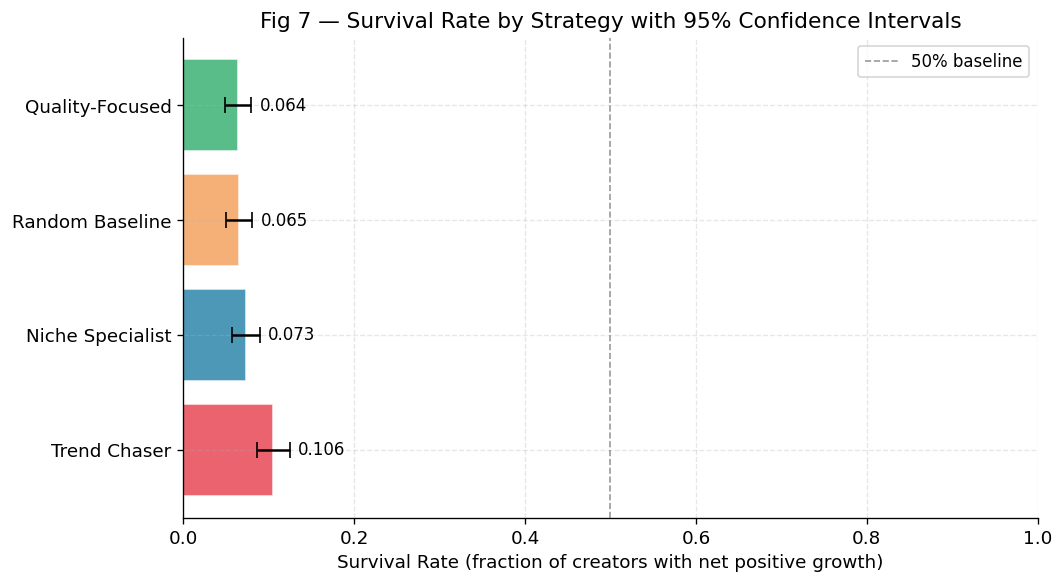
\includegraphics[width=0.72\linewidth]{fig7_survival_rate.png}
  \caption{\textbf{Survival rate differs by strategy even when mean followers do not.} The trend chaser has the highest probability of net-positive follower change over 60 weeks, consistent with a volume-driven mechanism offsetting churn \appref{A7}.}
  \label{fig:fig7}
\end{figure}

\subsection{Experiment 3: virality probability (simulation vs.\ theory)}
Virality is where strategy differentiation is strongest. Appendix A8 compares simulated viral rates to the analytical normal-approximation predictions from Appendix A5 \appref{A8}. Simulated viral rates are:
\[
\text{Quality-Focused } 1.0000,\quad
\text{Niche } 0.3990,\quad
\text{Random } 0.1980,\quad
\text{Trend Chaser } 0.0495
\]
\appref{A8}. These are cleanly separated by confidence intervals \appref{A11}. The theory predicts 1.0 for quality-focused and near-zero for trend chaser and random, with niche at 0.0703 \appref{A5}. The quality-focused match is exact; the others deviate upward, especially niche and random.

The deviation is explained by conditioning on trend alignment. The analytical model treats engagement probabilities as if they were evaluated at a fixed quality and topic baseline. In the simulation, when a trend is active and a creator aligns with it, share probability receives a multiplicative boost, shifting the engagement-score distribution upward and pushing many borderline cases above threshold \appref{A2b, A8}. That mechanism is strongest for mid-quality strategies (niche and random), and weaker for very high quality (already above threshold) or very low quality (still often below threshold).

\begin{figure}[t]
  \centering
  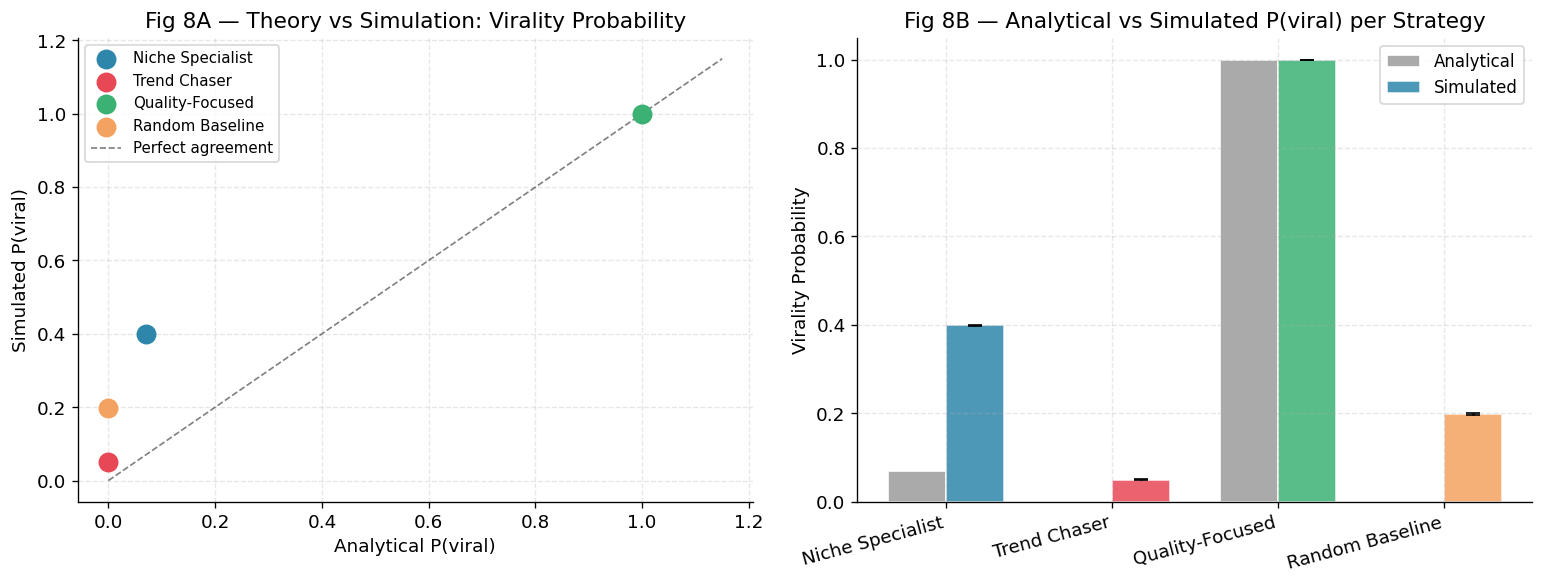
\includegraphics[width=0.98\linewidth]{fig8_virality.png}
  \caption{\textbf{Virality is strategy-dependent and theory is a partial benchmark.} All strategies lie above the theory diagonal except quality-focused, which sits at (1,1). Mid-quality strategies show the largest positive deviation because trend alignment boosts engagement in a way the independent normal approximation does not capture \appref{A5, A8}.}
  \label{fig:fig8}
\end{figure}

\subsection{Follow-up: viral rate by growth quartile}
Appendix A8b asks whether virality is the mechanism separating high-growth runs from low-growth runs \emph{within} a strategy \appref{A8b}. Runs are binned into quartiles by final followers (Q1 lowest to Q4 highest), and mean viral rates are computed per quartile.

The result is flat: within each strategy, viral rates are nearly constant across growth quartiles, and the Q4/Q1 ratios are essentially 1.00--1.01 \appref{A8b}. This matters because it rules out a tempting story: ``the top runs are the ones where more videos went viral.'' In this simulation, that is not the driver of run-to-run variation. Instead, run-level growth quartiles are dominated by differences in initial follower stocks produced by the tier-based initialization \appref{A1d, A2d}.

\begin{figure}[t]
  \centering
  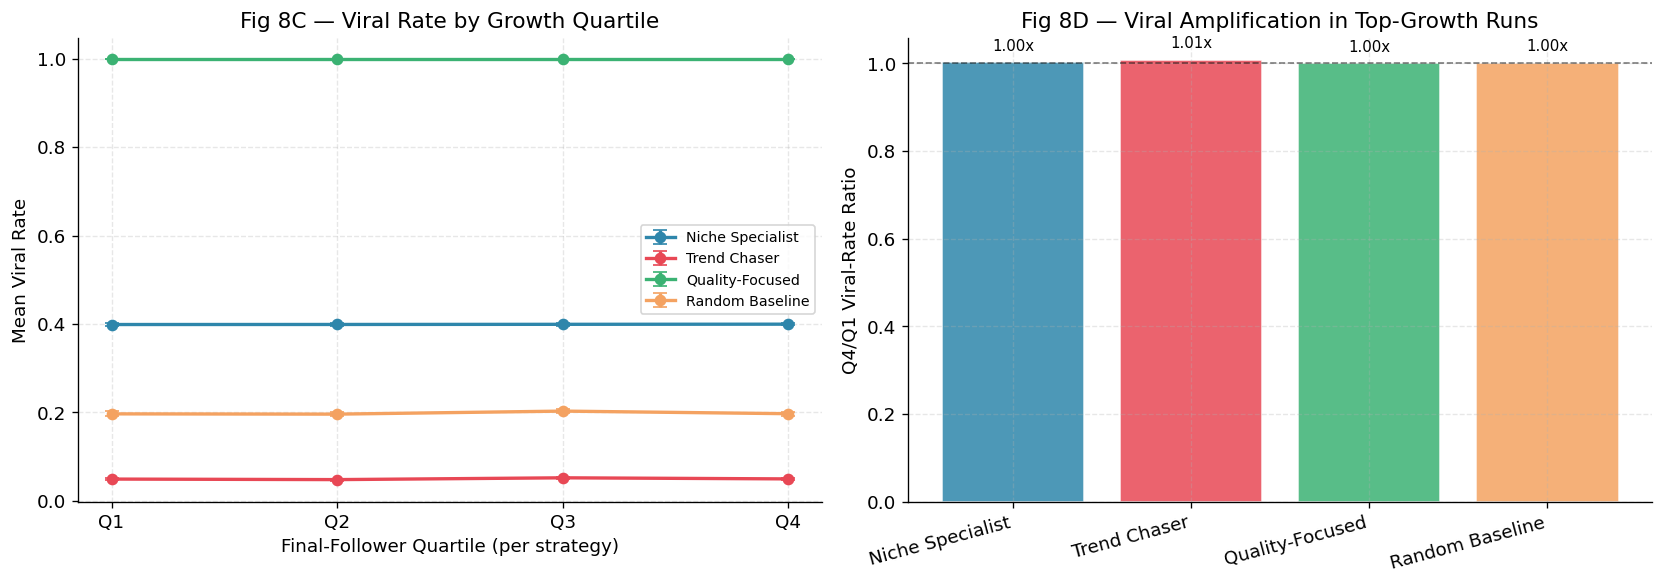
\includegraphics[width=0.98\linewidth]{fig8b_viral_growth_quartiles.png}
  \caption{\textbf{Within-strategy growth is not explained by within-strategy virality.} Viral rates are nearly constant from Q1 to Q4 within each strategy, and Q4/Q1 ratios are essentially 1. This supports the claim that initialization variance dominates run-level growth differences \appref{A8b}.}
  \label{fig:fig8b}
\end{figure}

\subsection{Experiment 4: inequality (Lorenz curves and Gini)}
Experiment 4 computes inequality within each run (across 30 creators) and compares simulated Lorenz curves to the real-data Lorenz curve \appref{A9}. The results show three consistent patterns:
\begin{enumerate}
  \item \(G_{\text{sim}}\approx 0.555\) to \(0.558\) for all strategies, essentially indistinguishable across strategies \appref{A9}.
  \item \(G_{\text{sim}} > G_{\text{theory}}\approx 0.319\) because the simulation inherits variance from the initial follower distribution in addition to multiplicative growth variance \appref{A5, A9}.
  \item \(G_{\text{sim}} \ll G_{\text{real}}=0.9086\). With only 30 creators per run, the simulation cannot represent the extreme top tail concentration visible in the 1{,}000-creator BrightData sample \appref{A1a, A9}.
\end{enumerate}

\begin{figure}[t]
  \centering
  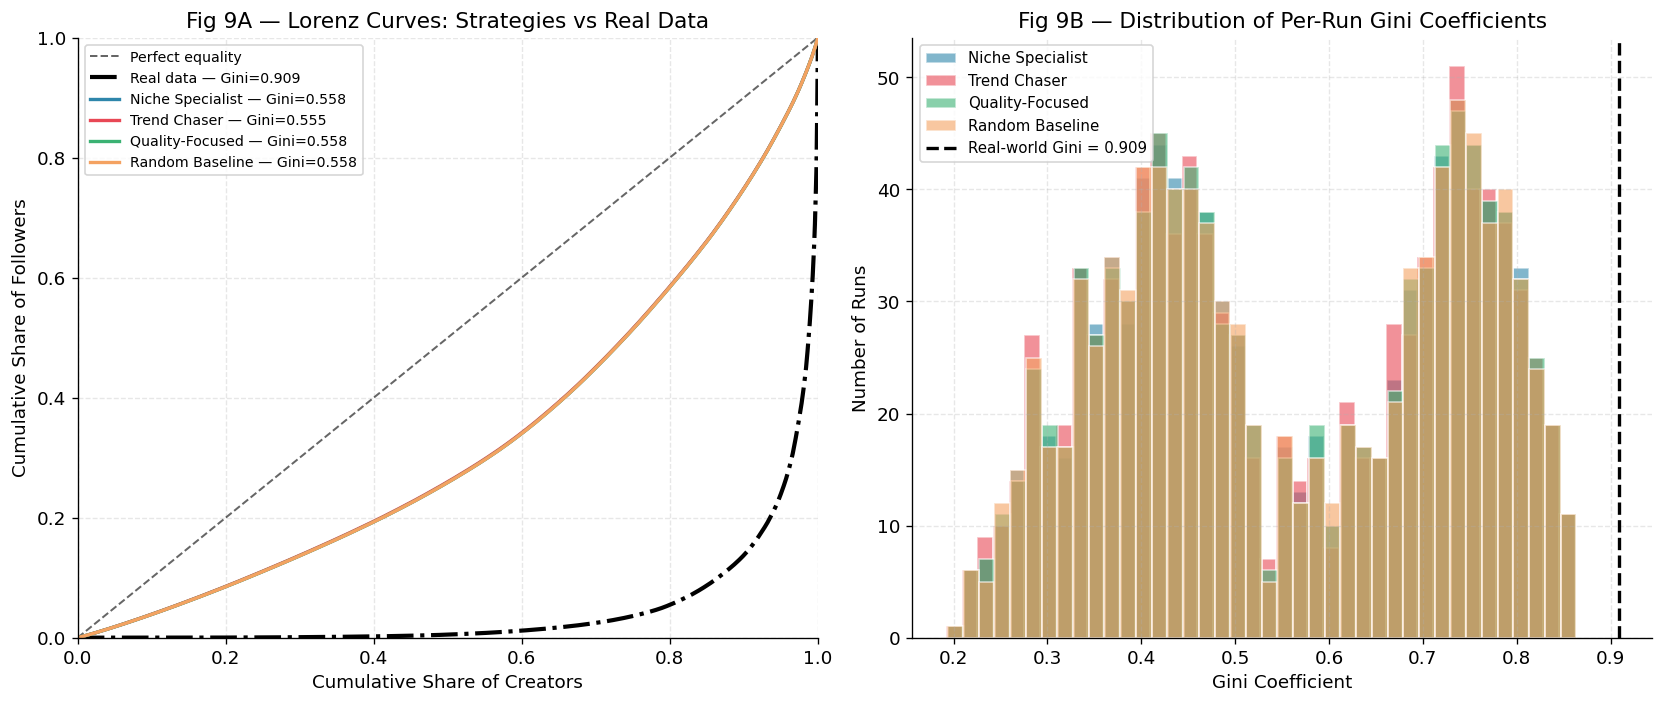
\includegraphics[width=0.95\linewidth]{fig9_lorenz_gini.png}
  \caption{\textbf{Inequality is high but strategy-independent in this model.} Simulated Lorenz curves overlap across strategies and lie between the equality diagonal and the real-data curve. The model produces substantial inequality (\(G_{\text{sim}}\approx 0.556\)) but cannot reach the extreme concentration in the real dataset at \(N=30\) creators \appref{A9}.}
  \label{fig:fig9}
\end{figure}

\subsection{Experiment 5: sensitivity analysis}
The sensitivity analysis varies trend frequency \(p_{\text{trend}}\in[0.02,0.30]\) and quality noise \(\sigma_q\in[0.05,0.35]\) on a \(5\times 5\) grid for two strategies (trend chaser and niche), using 30 runs per cell and a smaller simulation (10 creators, 30 steps) \appref{A10}. The output heatmaps show modest variation over the grid; both strategies produce similar spatial patterns, and the difference map contains both red and blue regions, indicating that neither strategy dominates uniformly across parameter regimes \appref{A10}.

Two points are worth being explicit about. First, the overall color intensity in both heatmaps is fairly light: across the tested ranges, mean final followers do not swing wildly. Second, the two heatmaps have visually similar patterning (dark blocks appear in the same locations), which suggests that the tested parameter variations shift both strategies in the same direction over much of the grid. The difference heatmap is therefore the meaningful diagnostic: it isolates where trend alignment and posting volume meaningfully change outcomes relative to niche consistency.

\begin{figure}[t]
  \centering
  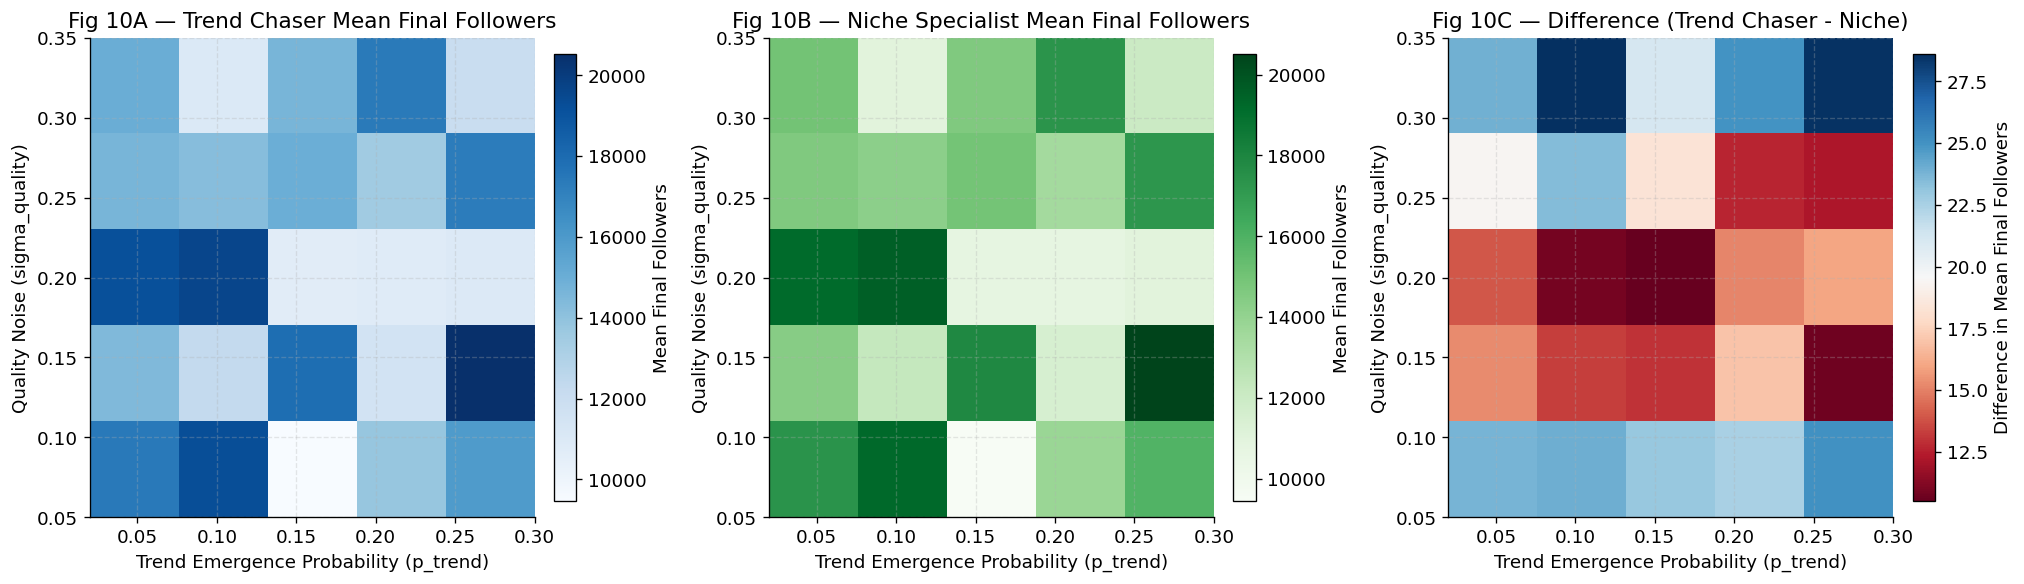
\includegraphics[width=1.0\linewidth]{fig10_sensitivity.png}
  \caption{\textbf{Sensitivity is modest; relative performance depends on regime.} Both strategies show similar broad patterns over \((p_{\text{trend}},\sigma_q)\), while the difference heatmap highlights regions where trend chasing outperforms niche consistency and vice versa \appref{A10}.}
  \label{fig:fig10}
\end{figure}

\subsection{Confidence intervals as a result, not a footnote}
Appendix A11 aggregates 95\% confidence intervals across key metrics \appref{A11}. The CI summary supports three conclusions:
\begin{enumerate}
  \item \textbf{Mean final followers are tied.} CI widths are about 1{,}101 followers and overlap heavily across strategies, so any ranking by mean final followers is not stable at \(N=1{,}000\) runs.
  \item \textbf{Survival rate differences are real but small.} Trend chaser's survival advantage over quality-focused is statistically clear because the CIs do not overlap.
  \item \textbf{Viral rate is the clearest differentiator.} Viral-rate CIs are tight and non-overlapping across the four strategies; quality-focused is effectively pinned at 1.0.
\end{enumerate}

\begin{figure}[t]
  \centering
  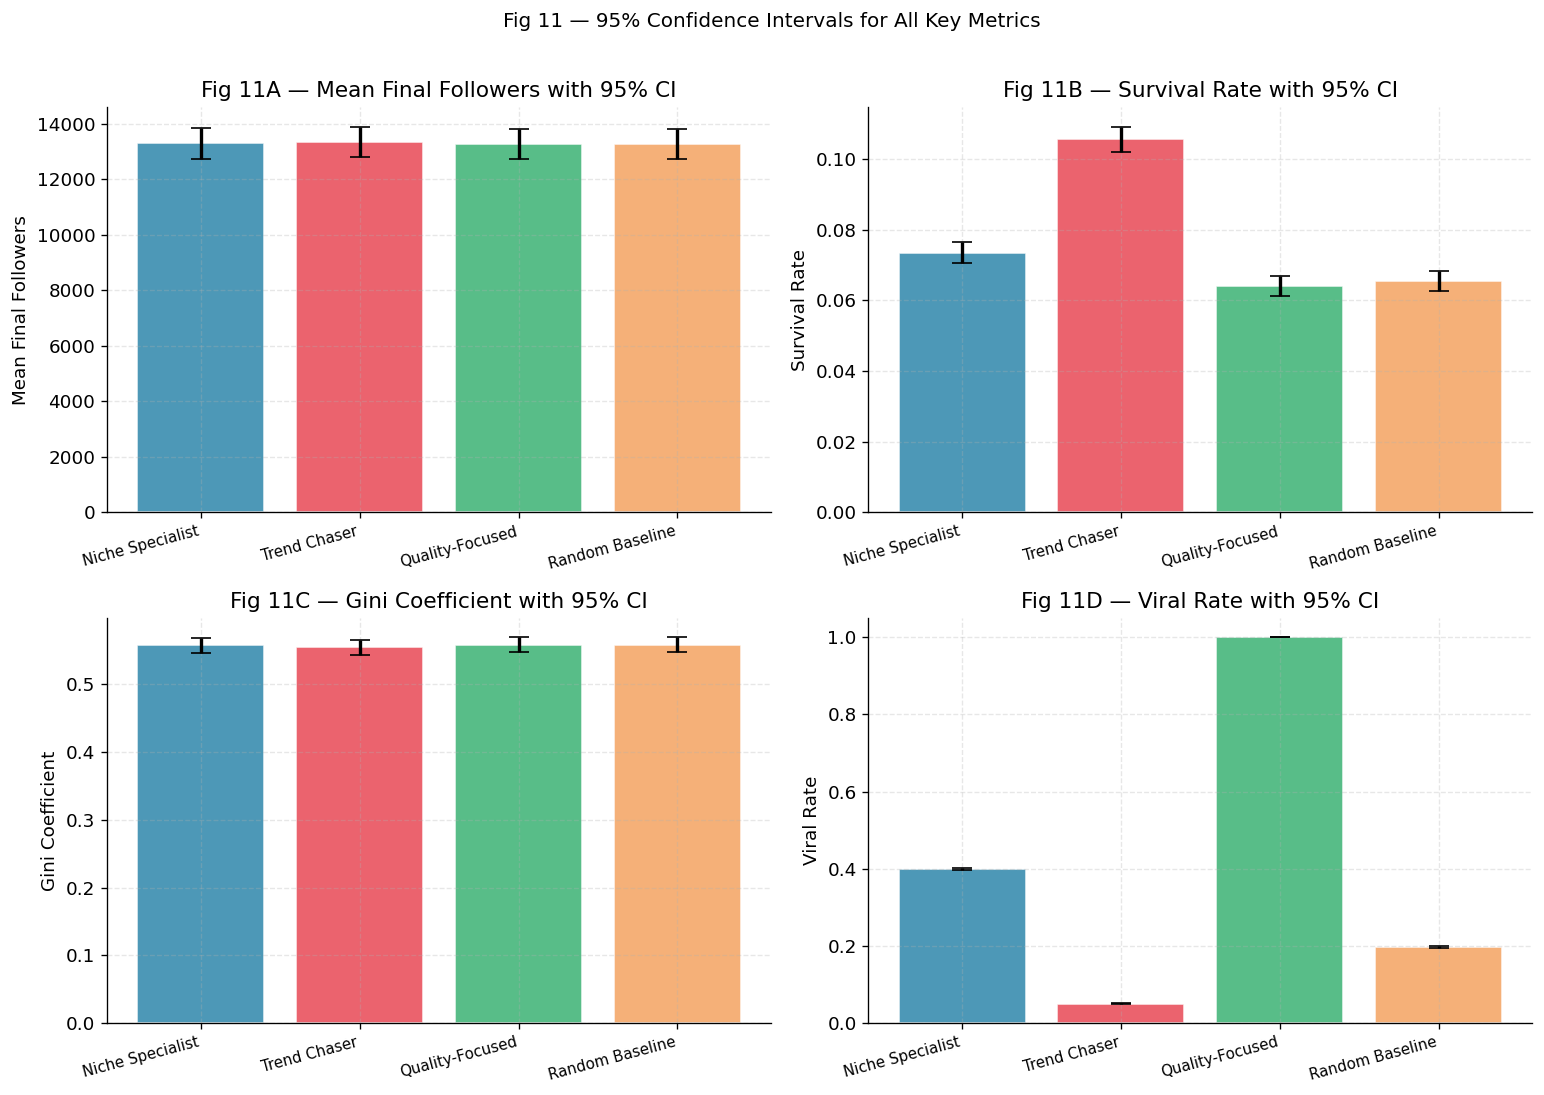
\includegraphics[width=0.88\linewidth]{fig11_confidence_intervals.png}
  \caption{\textbf{Confidence intervals summarize what is statistically distinguishable.} Viral rates separate strategies cleanly; survival rates separate trend chaser from the rest; mean final followers and Gini overlap across strategies \appref{A11}.}
  \label{fig:fig11}
\end{figure}

\section{Discussion and executive summary}
\subsection{Integrated interpretation}
The results separate cleanly into two categories: magnitude and mechanism. On magnitude, mean final followers are essentially unchanged across strategies \appref{A6, A11}. That is not a failure of plotting or insufficient Monte Carlo repetitions; it is the outcome of modeling choices that were made deliberately for realism. Creators start with a nontrivial follower stock drawn from tier distributions, and the churn term operates on that stock. In this regime, mean final followers are driven primarily by initialization and churn balance.

On mechanism, strategies differ sharply. Viral rate is highest for quality-focused creators (1.0), then niche (0.3990), then random (0.1980), then trend chaser (0.0495) \appref{A8}. Survival rate, however, ranks differently: trend chasing has the highest probability of net-positive mean follower change over 60 weeks \appref{A7}. The model implies two distinct ways to ``do well'' depending on the objective: maximize per-video viral probability (quality investment) or maximize the chance of not losing ground under churn (high posting volume with trend alignment).

Inequality is high but strategy-independent in the model: the simulated Gini is around 0.556 for all strategies \appref{A9}. The gap to the real-data Gini (0.9086) is best interpreted as a scale limitation. With only 30 creators per run, the simulation cannot express the extreme right tail concentration seen on the real platform. A larger agent population is the most direct path to testing whether the model's feedback loop can generate ultra-heavy tails.

\subsection{Executive summary (non-technical reader)}
This simulation compares four creator strategies over many randomized platform environments. On average, all four strategies end up with similar follower totals after 60 weeks. In the model, TikTok's baseline distribution gives every video a chance to reach a first audience, so no strategy has a decisive advantage on total followers alone.

Where strategies differ is \emph{how} they grow and how risky they are. A quality-focused creator goes ``viral'' on almost every post in this model, meaning each post earns amplified distribution. A trend-chasing creator rarely has any single post go viral, but posts more often and gets periodic boosts when aligned with a trend; that volume makes them most likely to end the year with more followers than they started with. For a client who wants reliability and wants to avoid net losses, the model favors a trend-aware, higher-volume schedule. For a client aiming for viral reach per post, the model favors quality investment.

\subsection{Limitations and future work}
Three limitations are directly tied to the results:
\begin{enumerate}
  \item \textbf{No learning or skill acquisition.} Quality is fixed within-run, so the model cannot represent creators improving over time. Adding a slow quality update rule would test whether quality-focused remains dominant on virality when learning is possible.
  \item \textbf{No user network structure.} Users are sampled from a static preference distribution, so community-driven cascades are absent. Introducing even a simple community graph would likely raise inequality and could specifically advantage niche specialists.
  \item \textbf{Small creator population per run.} With 30 creators, the Lorenz curve cannot develop the extreme top tail seen in real data. Scaling to 500--1{,}000 creators per run would be computationally heavier but would give a cleaner inequality comparison.
\end{enumerate}

\section{References}
\begin{thebibliography}{9}
\bibitem{berry1941}
Berry, A.\ C.\ (1941).
The accuracy of the Gaussian approximation to the sum of independent variates.
\textit{Transactions of the American Mathematical Society}, 49(1), 122--136.

\bibitem{brightdata}
Bright Data.
\textit{TikTok user profiles dataset} (CSV; creator-level sample).
Used for follower distribution and Lorenz/Gini calibration \appref{A1a}.

\bibitem{kagglehashtags}
Kaggle (CC0).
\textit{TikTok popular hashtags dataset} (XLSX; video-level engagement by hashtag).
Used for topic multipliers \appref{A1b}.

\bibitem{hypeauditor}
HypeAuditor (2026).
\textit{State of Influencer Marketing 2026}.
Used for tier distribution and benchmark engagement by tier \appref{A1d}.

\bibitem{googletrends}
Google Trends.
Weekly interest time series for Sea Shanty (Nov 2020--Apr 2021), Corn Kid (Aug--Dec 2022), Brat Summer (May--Oct 2024), and Demure (Jul--Nov 2024).
Used for log-normal lifecycle fitting \appref{A1c}.
\end{thebibliography}

\end{document}

